\subsection{A haptic cue: when, from which signal, with which threshold (Q4)}
\label{sec:res-haptic}

The cue is meant for the \emph{trailing} limb, which crosses the obstacle without seeing it. Its deadline is the moment the trailing
toe leaves the floor (camera lift-off); all times below are relative to that moment.

\subsubsection{Timeline of a crossing}

Table~\ref{tab:timeline} gives the median times. The leading toe leaves the floor 817\,ms before the deadline, the leading foot
reaches its apex at $-450$\,ms (IQR $-517$ to $-350$) and lands at $-200$\,ms (IQR $-300$ to $-33$). Once the trailing toe has left
the floor it is over the obstacle centre only 184\,ms later, too fast for any reaction. In 22\,\% of the crossings the trailing toe
even leaves the floor before the leading foot has landed (Table~\ref{tab:cueing}). The cue therefore has to come from the leading
limb, around its apex.

\begin{table}[htbp]
\centering
\caption{Timeline of a crossing relative to the trailing toe lift-off (deadline of a cue for the trailing limb).}
\label{tab:timeline}
\begin{adjustbox}{max width=\textwidth}
{\footnotesize
\begin{tabular}{p{7.4cm}rrr}
\toprule
\textbf{event} & \textbf{median (ms)} & \textbf{IQR (ms)} & \textbf{crossings} \\
\midrule
leading toe lift-off (camera) & $-$817 & $-$912 to $-$733 & 259 \\
leading toe-off event (IMU, step 4) & $-$733 & $-$817 to $-$621 & 259 \\
leading foot apex (IMU) & $-$450 & $-$517 to $-$350 & 259 \\
leading toe over the obstacle centre (camera) & $-$505 & $-$574 to $-$402 & 259 \\
leading heel-strike (landing, IMU) & $-$200 & $-$300 to $-$33 & 259 \\
trailing toe lift-off (camera) = deadline & +0 & +0 to +0 & 259 \\
trailing toe over the obstacle centre (camera) & +184 & +147 to +254 & 259 \\
trailing toe-off event (IMU, step 4) & +233 & +167 to +367 & 259 \\
trailing foot apex (IMU) & +300 & +233 to +433 & 259 \\
trailing heel-strike (landing, IMU) & +633 & +533 to +783 & 259 \\
\bottomrule
\end{tabular}
}
\end{adjustbox}

\end{table}

\begin{table}[htbp]
\centering
\caption{Cueing window: time from the leading-limb events to the trailing toe lift-off, overall and per height; \% $>$ 0 = share of
crossings in which the event comes before the lift-off.}
\label{tab:cueing}
\begin{adjustbox}{max width=\textwidth}
{\footnotesize
\begin{tabular}{lrrrrrrr}
\toprule
\textbf{interval} & \textbf{n} & \textbf{median} & \textbf{IQR} & \textbf{\% $>$ 0} & \textbf{H1 median} & \textbf{H2 median} & \textbf{H3 median} \\
\midrule
lead toe-off $\rightarrow$ trailing lift-off & 259 & 733 & 625 to 817 & 100\% & 658 & 783 & 800 \\
lead foot apex $\rightarrow$ trailing lift-off & 259 & 450 & 350 to 517 & 100\% & 383 & 483 & 450 \\
lead landing $\rightarrow$ trailing lift-off & 259 & 200 & 33 to 300 & 78\% & 133 & 233 & 200 \\
trailing lift-off $\rightarrow$ trailing foot apex & 259 & 300 & 233 to 433 & 100\% & 275 & 283 & 367 \\
trailing lift-off $\rightarrow$ step-4 trailing toe-off event (IMU) & 259 & 233 & 167 to 367 & 100\% & 200 & 217 & 317 \\
\bottomrule
\end{tabular}
}
\end{adjustbox}

\end{table}

\subsubsection{Detecting the crossing from one signal}

A single threshold on one leading-limb signal, referenced to the person's normal walking, detects the crossing early and reliably
(Table~\ref{tab:detect}): leading-thigh tilt more than 5.6\textdegree{} above normal walking at 30\,\% of the leading swing (573\,ms
before the deadline) gives 97\,\% sensitivity and 98\,\% specificity; leading-foot height more than 18.6\,mm above normal walking at
18\,\% of the swing (640\,ms before) gives 99\,\% and 98\,\%. Both reach at least 90\,\% sensitivity and specificity from 10\,\% and
4\,\% of the leading swing (682 and 713\,ms before the deadline). The leading shank and foot tilt are poor detectors. The trailing
limb detects equally well but only after its toe has left the floor. (Specificity is estimated on 39--46 level strides only; the
stride-based detector of Section~\ref{sec:res-cue}, tested on all 7250 strides, has about 3 false detections per session.)

\begin{table}[htbp]
\centering
\caption{Crossing vs level stride from one signal (vs normal walking): nested sensitivity / specificity, chosen moment and threshold,
and the earliest moment at which a fixed-moment rule reaches at least 90\,\% of both.}
\label{tab:detect}
\begin{adjustbox}{max width=\textwidth}
{\scriptsize
\begin{tabular}{llrrrr}
\toprule
\textbf{limb} & \textbf{signal} & \textbf{nested: sensitivity / specificity} & \textbf{moment chosen (median, \% swing; ms vs trailing lift-off)} & \textbf{threshold (vs normal walking)} & \textbf{earliest moment with both $\geq$ 90\%} \\
\midrule
lead & thigh tilt & 97\% / 98\% & 30\% ($-$573 ms) & $\geq$ +5.6 deg & 10\% ($-$682 ms) \\
lead & shank tilt & 61\% / 88\% & 14\% ($-$661 ms) & $\leq$ $-$3.0 deg & - \\
lead & foot tilt & 66\% / 88\% & 46\% ($-$479 ms) & $\geq$ +4.7 deg & - \\
lead & foot height & 99\% / 98\% & 18\% ($-$640 ms) & $\geq$ +18.6 mm & 4\% ($-$713 ms) \\
trail & thigh tilt & 93\% / 92\% & 46\% (+410 ms) & $\geq$ +4.3 deg & 32\% (+356 ms) \\
trail & shank tilt & 99\% / 98\% & 0\% (+233 ms) & $\leq$ $-$6.4 deg & 0\% (+233 ms) \\
trail & foot tilt & 95\% / 98\% & 14\% (+285 ms) & $\leq$ $-$7.7 deg & 0\% (+233 ms) \\
trail & foot height & 99\% / 98\% & 8\% (+261 ms) & $\geq$ +19.9 mm & 0\% (+233 ms) \\
\bottomrule
\end{tabular}
}
\end{adjustbox}

\end{table}

\subsubsection{Grading the height from one signal}

With two thresholds on one signal at one moment of the swing (Table~\ref{tab:grade}), the best leading-limb signal is the foot height
relative to the person's typical crossing: 73.4\,\% at 46\,\% of the leading swing (479\,ms before the deadline). The leading thigh
gives 63.9\,\% (72\,\% of the swing, 345\,ms before). Referenced only to normal walking (no crossing of the person yet) they give 45
and 52\,\%, because the personal margin is not removed. The leading shank and foot tilt do not grade the height. The trailing shank
(81.4\,\%) and trailing foot height (82.3\,\%) grade the height best, but only 250--300\,ms after the trailing toe has left the floor.
The multi-feature real-time model of Section~\ref{sec:res-cue} (71--76\,\% correct cues) is therefore comparable to the best single
leading-limb signal; the after-the-fact recognition with both limbs is much better (92\,\%).

\begin{table}[htbp]
\centering
\caption{Height from one signal at one moment of the swing (two ordered thresholds): nested accuracy, chosen moment and the device
thresholds (refitted on all participants).}
\label{tab:grade}
\begin{adjustbox}{max width=\textwidth}
{\scriptsize
\begin{tabular}{lllrrr}
\toprule
\textbf{limb} & \textbf{signal} & \textbf{reference} & \textbf{nested accuracy (95\% CI)} & \textbf{moment (\% swing; ms vs trailing lift-off)} & \textbf{thresholds H1/H2, H2/H3} \\
\midrule
lead & thigh tilt & vs normal walking & 52.4\% (40--64) & 42\% ($-$507 ms) & +43.3, +47.7 deg (rises with height) \\
lead & thigh tilt & person-centred & 63.9\% (52--74) & 72\% ($-$345 ms) & $-$3.2, +5.0 deg (rises with height) \\
lead & shank tilt & vs normal walking & 29.7\% (26--34) & 12\% ($-$671 ms) & $-$4.9, $-$10.4 deg (falls with height) \\
lead & shank tilt & person-centred & 38.9\% (30--47) & 48\% ($-$469 ms) & $-$5.0, +4.8 deg (rises with height) \\
lead & foot tilt & vs normal walking & 25.2\% (21--29) & 98\% ($-$210 ms) & +6.4, +3.8 deg (falls with height) \\
lead & foot tilt & person-centred & 43.2\% (37--49) & 48\% ($-$469 ms) & $-$4.7, +3.4 deg (rises with height) \\
lead & foot height & vs normal walking & 45.4\% (38--54) & 30\% ($-$573 ms) & +220.3, +295.2 mm (rises with height) \\
lead & foot height & person-centred & 73.4\% (62--82) & 46\% ($-$479 ms) & $-$35.8, +38.6 mm (rises with height) \\
trail & thigh tilt & vs normal walking & 36.3\% (34--40) & 50\% (+425 ms) & +18.4, +24.8 deg (rises with height) \\
trail & thigh tilt & person-centred & 35.0\% (26--44) & 42\% (+394 ms) & +1.4, +3.9 deg (rises with height) \\
trail & shank tilt & vs normal walking & 68.6\% (55--80) & 6\% (+254 ms) & $-$33.6, $-$46.2 deg (falls with height) \\
trail & shank tilt & person-centred & 81.4\% (72--89) & 6\% (+254 ms) & +6.5, $-$3.9 deg (falls with height) \\
trail & foot tilt & vs normal walking & 45.7\% (36--55) & 4\% (+247 ms) & $-$20.9, $-$26.9 deg (falls with height) \\
trail & foot tilt & person-centred & 60.2\% (51--67) & 4\% (+247 ms) & +4.1, $-$4.3 deg (falls with height) \\
trail & foot height & vs normal walking & 55.8\% (44--69) & 28\% (+341 ms) & +269.0, +352.6 mm (rises with height) \\
trail & foot height & person-centred & 82.3\% (74--89) & 16\% (+292 ms) & $-$46.6, +54.0 mm (rises with height) \\
\bottomrule
\end{tabular}
}
\end{adjustbox}

\end{table}

\subsubsection{How much: the extra angle and lift per height}

Table~\ref{tab:dose} gives, at the most informative moment of each signal, the mean value relative to normal walking for each height,
the change per cm of obstacle and the crossing-to-crossing SD. At 60\,\% of the leading swing (410\,ms before the deadline) the
leading thigh is flexed 35\textdegree{}, 46\textdegree{} and 53\textdegree{} more than in normal walking for H1, H2 and H3 (about
1\textdegree{} per cm, crossing-to-crossing SD 6.6\textdegree{}); the leading foot is 204, 298 and 361\,mm higher at its apex
(8.6\,mm per cm, SD 48\,mm). The trailing shank tilts backward 31\textdegree{}, 46\textdegree{} and 55\textdegree{} more at push-off
($-1.3$\textdegree{} per cm, SD 5.6\textdegree{}) and the trailing foot rises 237, 352 and 436\,mm (10.9\,mm per cm, SD 36\,mm). The
spread between participants (the $\pm$ values, 10--14\textdegree{} for the thigh, about 60--85\,mm for the foot height) is as large as the
step between two heights, so useful thresholds must be personal.

\begin{table}[htbp]
\centering
\caption{Extra angle and lift per height relative to normal walking (mean of the participant means $\pm$ SD across participants),
change per cm of obstacle, and crossing-to-crossing SD within a participant and obstacle.}
\label{tab:dose}
\begin{adjustbox}{max width=\textwidth}
{\scriptsize
\begin{tabular}{llrrrrrrr}
\toprule
\textbf{limb} & \textbf{signal} & \textbf{moment (\% swing; ms vs trailing lift-off)} & \textbf{$\eta^2$} & \textbf{H1} & \textbf{H2} & \textbf{H3} & \textbf{per cm of obstacle} & \textbf{crossing-to-crossing SD} \\
\midrule
lead & thigh tilt & 60\% ($-$410 ms) & 0.45 & +35.4 $\pm$ 9.9 & +45.8 $\pm$ 11.7 & +52.9 $\pm$ 13.5 & +0.95 deg & 6.6 deg \\
lead & shank tilt & 90\% ($-$248 ms) & 0.04 & $-$0.1 $\pm$ 7.9 & $-$3.2 $\pm$ 13.0 & $-$3.4 $\pm$ 12.9 & $-$0.15 deg & 5.8 deg \\
lead & foot tilt & 90\% ($-$248 ms) & 0.07 & +3.5 $\pm$ 11.1 & $-$0.7 $\pm$ 11.8 & $-$2.7 $\pm$ 11.6 & $-$0.29 deg & 6.4 deg \\
lead & foot height & 46\% ($-$479 ms) & 0.59 & +203.9 $\pm$ 65.5 & +297.6 $\pm$ 65.1 & +360.6 $\pm$ 75.9 & +8.62 mm & 47.6 mm \\
trail & thigh tilt & 44\% (+402 ms) & 0.14 & +13.4 $\pm$ 4.6 & +16.3 $\pm$ 7.0 & +18.4 $\pm$ 8.5 & +0.28 deg & 3.9 deg \\
trail & shank tilt & 4\% (+247 ms) & 0.65 & $-$31.1 $\pm$ 14.1 & $-$45.6 $\pm$ 13.5 & $-$54.7 $\pm$ 9.3 & $-$1.30 deg & 5.6 deg \\
trail & foot tilt & 2\% (+240 ms) & 0.35 & $-$18.1 $\pm$ 11.6 & $-$28.1 $\pm$ 12.0 & $-$33.7 $\pm$ 10.6 & $-$0.85 deg & 7.4 deg \\
trail & foot height & 18\% (+299 ms) & 0.75 & +237.4 $\pm$ 84.4 & +352.3 $\pm$ 70.5 & +436.0 $\pm$ 59.2 & +10.89 mm & 36.1 mm \\
\bottomrule
\end{tabular}
}
\end{adjustbox}

\end{table}

\subsubsection{Real time: fixed times before the deadline}

On the time-aligned signals (Table~\ref{tab:realtime}, Figure~\ref{fig:haptic}), the leading foot height is again the best single
signal (person-centred 72\,\%, best about 470\,ms before the deadline), and the leading thigh gives about 60\,\%. Every trailing-limb
signal stays near chance (41--51\,\%) before the lift-off: the trailing limb shows no sign of the obstacle height before it leaves the
floor. Fixed clock times blur the signals, because the timing of the crossing varies from one crossing to the next; a device should
trigger on leading-limb events (toe-off, apex) rather than on a fixed clock. Table~\ref{tab:rules} lists the corresponding rules
referenced to normal walking for a cue that must be ready 300\,ms before the deadline.

\begin{table}[htbp]
\centering
\caption{Height from one signal at fixed times before the trailing toe lift-off: nested accuracy for each cue deadline (median chosen
time in brackets).}
\label{tab:realtime}
\begin{adjustbox}{max width=\textwidth}
{\scriptsize
\begin{tabular}{lllrrrrr}
\toprule
\textbf{limb} & \textbf{signal} & \textbf{reference} & \textbf{data up to 500 ms before} & \textbf{data up to 300 ms before} & \textbf{data up to 200 ms before} & \textbf{data up to 100 ms before} & \textbf{up to the lift-off} \\
\midrule
lead & thigh tilt & vs normal walking & 39\% ($-$500 ms) & 55\% ($-$417 ms) & 55\% ($-$417 ms) & 55\% ($-$417 ms) & 55\% ($-$417 ms) \\
lead & thigh tilt & person-centred & 61\% ($-$500 ms) & 60\% ($-$417 ms) & 60\% ($-$417 ms) & 60\% ($-$417 ms) & 60\% ($-$417 ms) \\
lead & shank tilt & vs normal walking & 33\% ($-$967 ms) & 33\% ($-$967 ms) & 33\% ($-$967 ms) & 33\% ($-$967 ms) & 33\% ($-$967 ms) \\
lead & shank tilt & person-centred & 49\% ($-$817 ms) & 49\% ($-$817 ms) & 49\% ($-$817 ms) & 49\% ($-$817 ms) & 49\% ($-$817 ms) \\
lead & foot tilt & vs normal walking & 39\% ($-$900 ms) & 39\% ($-$900 ms) & 39\% ($-$900 ms) & 39\% ($-$900 ms) & 39\% ($-$900 ms) \\
lead & foot tilt & person-centred & 38\% ($-$950 ms) & 38\% ($-$950 ms) & 38\% ($-$950 ms) & 38\% ($-$950 ms) & 38\% ($-$950 ms) \\
lead & foot height & vs normal walking & 49\% ($-$500 ms) & 54\% ($-$450 ms) & 54\% ($-$450 ms) & 54\% ($-$450 ms) & 54\% ($-$450 ms) \\
lead & foot height & person-centred & 72\% ($-$500 ms) & 72\% ($-$467 ms) & 72\% ($-$467 ms) & 72\% ($-$467 ms) & 72\% ($-$467 ms) \\
trail & thigh tilt & vs normal walking & 41\% ($-$1333 ms) & 41\% ($-$1333 ms) & 41\% ($-$1333 ms) & 41\% ($-$1333 ms) & 41\% ($-$1333 ms) \\
trail & thigh tilt & person-centred & 51\% ($-$1217 ms) & 51\% ($-$1217 ms) & 51\% ($-$1217 ms) & 51\% ($-$1217 ms) & 51\% ($-$1217 ms) \\
trail & shank tilt & vs normal walking & 43\% ($-$1500 ms) & 43\% ($-$1500 ms) & 43\% ($-$1500 ms) & 43\% ($-$1500 ms) & 43\% ($-$1500 ms) \\
trail & shank tilt & person-centred & 42\% ($-$1475 ms) & 42\% ($-$1475 ms) & 42\% ($-$1475 ms) & 42\% ($-$1475 ms) & 42\% ($-$1475 ms) \\
trail & foot tilt & vs normal walking & 41\% ($-$1450 ms) & 41\% ($-$1450 ms) & 41\% ($-$1450 ms) & 41\% ($-$1450 ms) & 41\% ($-$1450 ms) \\
trail & foot tilt & person-centred & 46\% ($-$1467 ms) & 46\% ($-$1467 ms) & 46\% ($-$1467 ms) & 46\% ($-$1467 ms) & 46\% ($-$1467 ms) \\
trail & foot height & vs normal walking & 43\% ($-$1417 ms) & 43\% ($-$1417 ms) & 43\% ($-$1417 ms) & 43\% ($-$1417 ms) & 43\% ($-$1417 ms) \\
trail & foot height & person-centred & 50\% ($-$1383 ms) & 50\% ($-$1383 ms) & 50\% ($-$1383 ms) & 50\% ($-$1383 ms) & 50\% ($-$1383 ms) \\
\bottomrule
\end{tabular}
}
\end{adjustbox}

\end{table}

\begin{table}[htbp]
\centering
\caption{Single-signal rules for a cue ready 300\,ms before the trailing toe lift-off (referenced to normal walking; refitted on all
participants).}
\label{tab:rules}
\begin{adjustbox}{max width=\textwidth}
{\scriptsize
\begin{tabular}{llrrrlr}
\toprule
\textbf{limb} & \textbf{signal} & \textbf{moment (ms vs lift-off)} & \textbf{H1/H2 threshold} & \textbf{H2/H3 threshold} & \textbf{direction} & \textbf{accuracy on left-out participants} \\
\midrule
lead & thigh tilt & $-$417 & +34.4 deg & +45.5 deg & higher obstacle = larger value & 55\% \\
lead & shank tilt & $-$1133 & +0.9 deg & $-$10.6 deg & higher obstacle = smaller value & 33\% \\
lead & foot tilt & $-$850 & $-$23.5 deg & $-$44.1 deg & higher obstacle = smaller value & 39\% \\
lead & foot height & $-$450 & +230.8 mm & +325.4 mm & higher obstacle = larger value & 54\% \\
trail & thigh tilt & $-$1333 & +15.9 deg & +31.3 deg & higher obstacle = larger value & 41\% \\
trail & shank tilt & $-$1500 & $-$4.3 deg & $-$26.3 deg & higher obstacle = smaller value & 43\% \\
trail & foot tilt & $-$1450 & $-$4.8 deg & $-$46.2 deg & higher obstacle = smaller value & 41\% \\
trail & foot height & $-$1433 & +7.5 mm & +21.1 mm & higher obstacle = larger value & 43\% \\
\bottomrule
\end{tabular}
}
\end{adjustbox}

\end{table}

Figure~\ref{fig:haptic} shows the accuracy of one signal over time and Figure~\ref{fig:hapticcurves} the signals behind it: the
leading thigh tilt and foot height separate the three heights from about 0.6--0.8\,s before the trailing toe lift-off, whereas the
trailing shank and foot separate them only after it.

\begin{figure}[htbp]
\centering
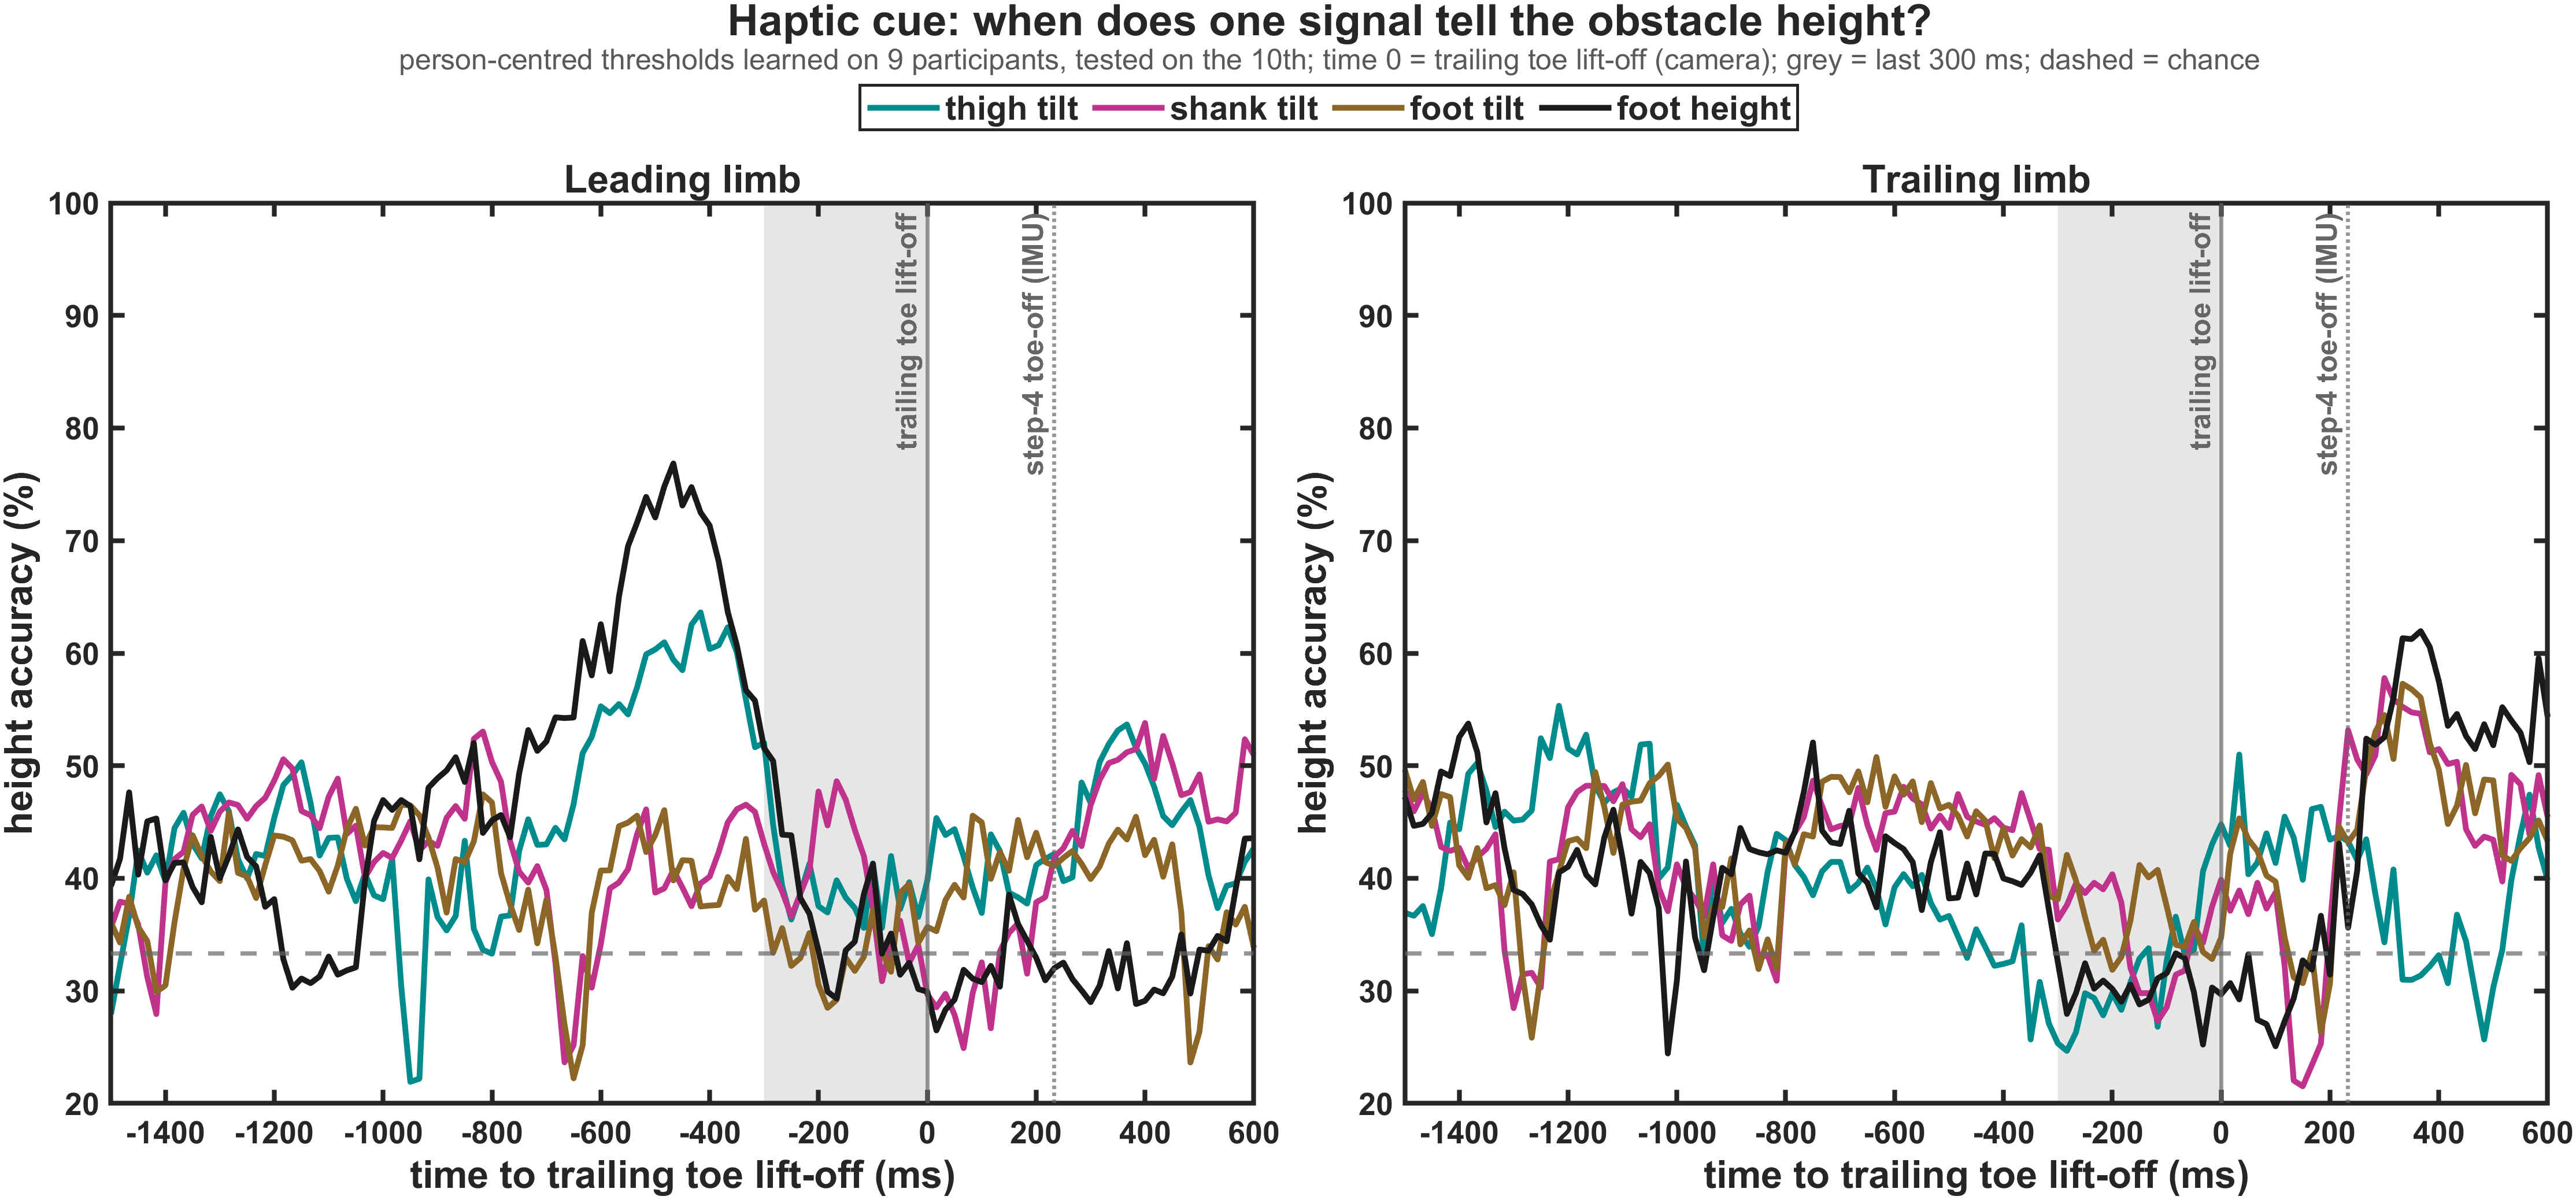
\includegraphics[width=\textwidth]{fig_haptic.png}
\caption{Haptic timing: height accuracy from one signal with person-centred thresholds (learned on nine participants, tested on the
tenth) at each time relative to the trailing toe lift-off, for the leading (left) and the trailing (right) limb. Grey = last 300\,ms;
dotted = median step-4 trailing toe-off event (IMU); dashed = chance.}
\label{fig:haptic}
\end{figure}

\begin{figure}[htbp]
\centering
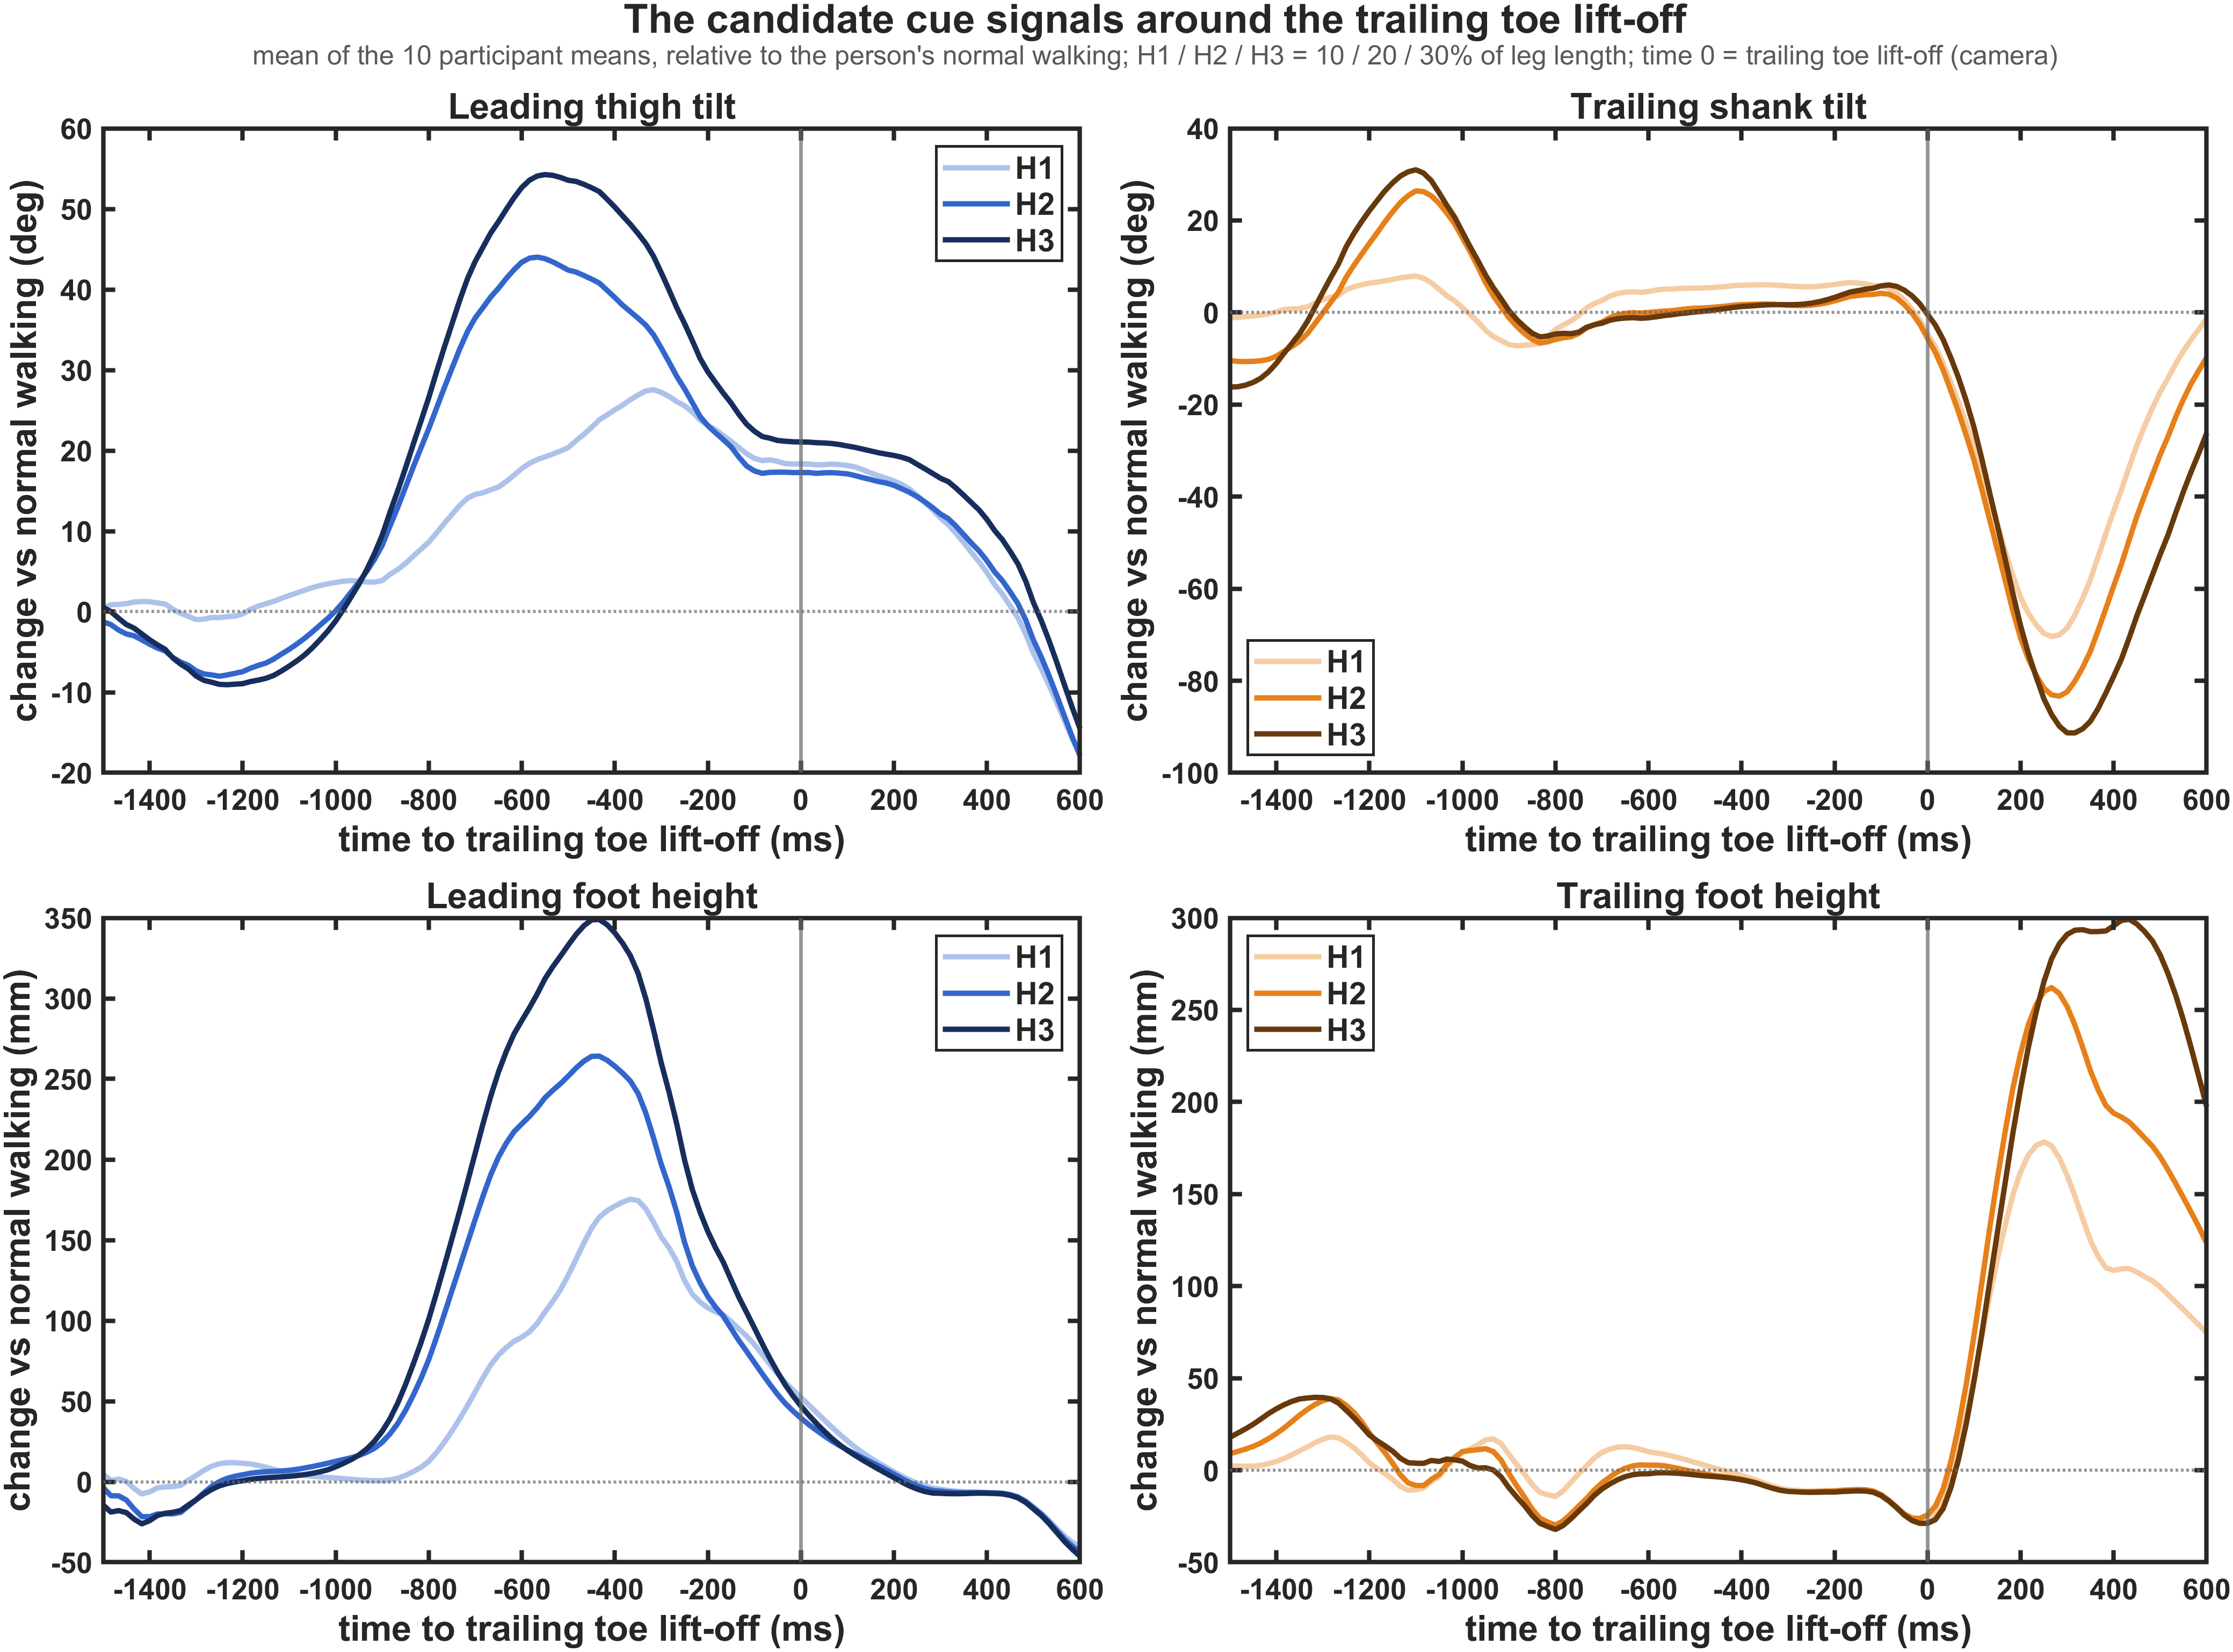
\includegraphics[width=\textwidth]{fig_haptic_curves.png}
\caption{The candidate cue signals around the trailing toe lift-off, relative to the person's normal walking: leading thigh tilt,
trailing shank tilt, leading and trailing foot height. Mean of the 10 participant means per obstacle height (light to dark =
H1 to H3); vertical line = trailing toe lift-off.}
\label{fig:hapticcurves}
\end{figure}
